\section{Placer des points (2 points)}

\begin{questions}
	\question[1] Reproduire une figure semblable à celle ci dessous. Les dimensions n'ont pas d'importance.
	
	

	\question[2] Placer les points $B$, $C$, $D$ et $E$ %\textbf{sur cette figure}
	, sachant que :
	
	\begin{multicols}{2}
		
		\begin{center}
			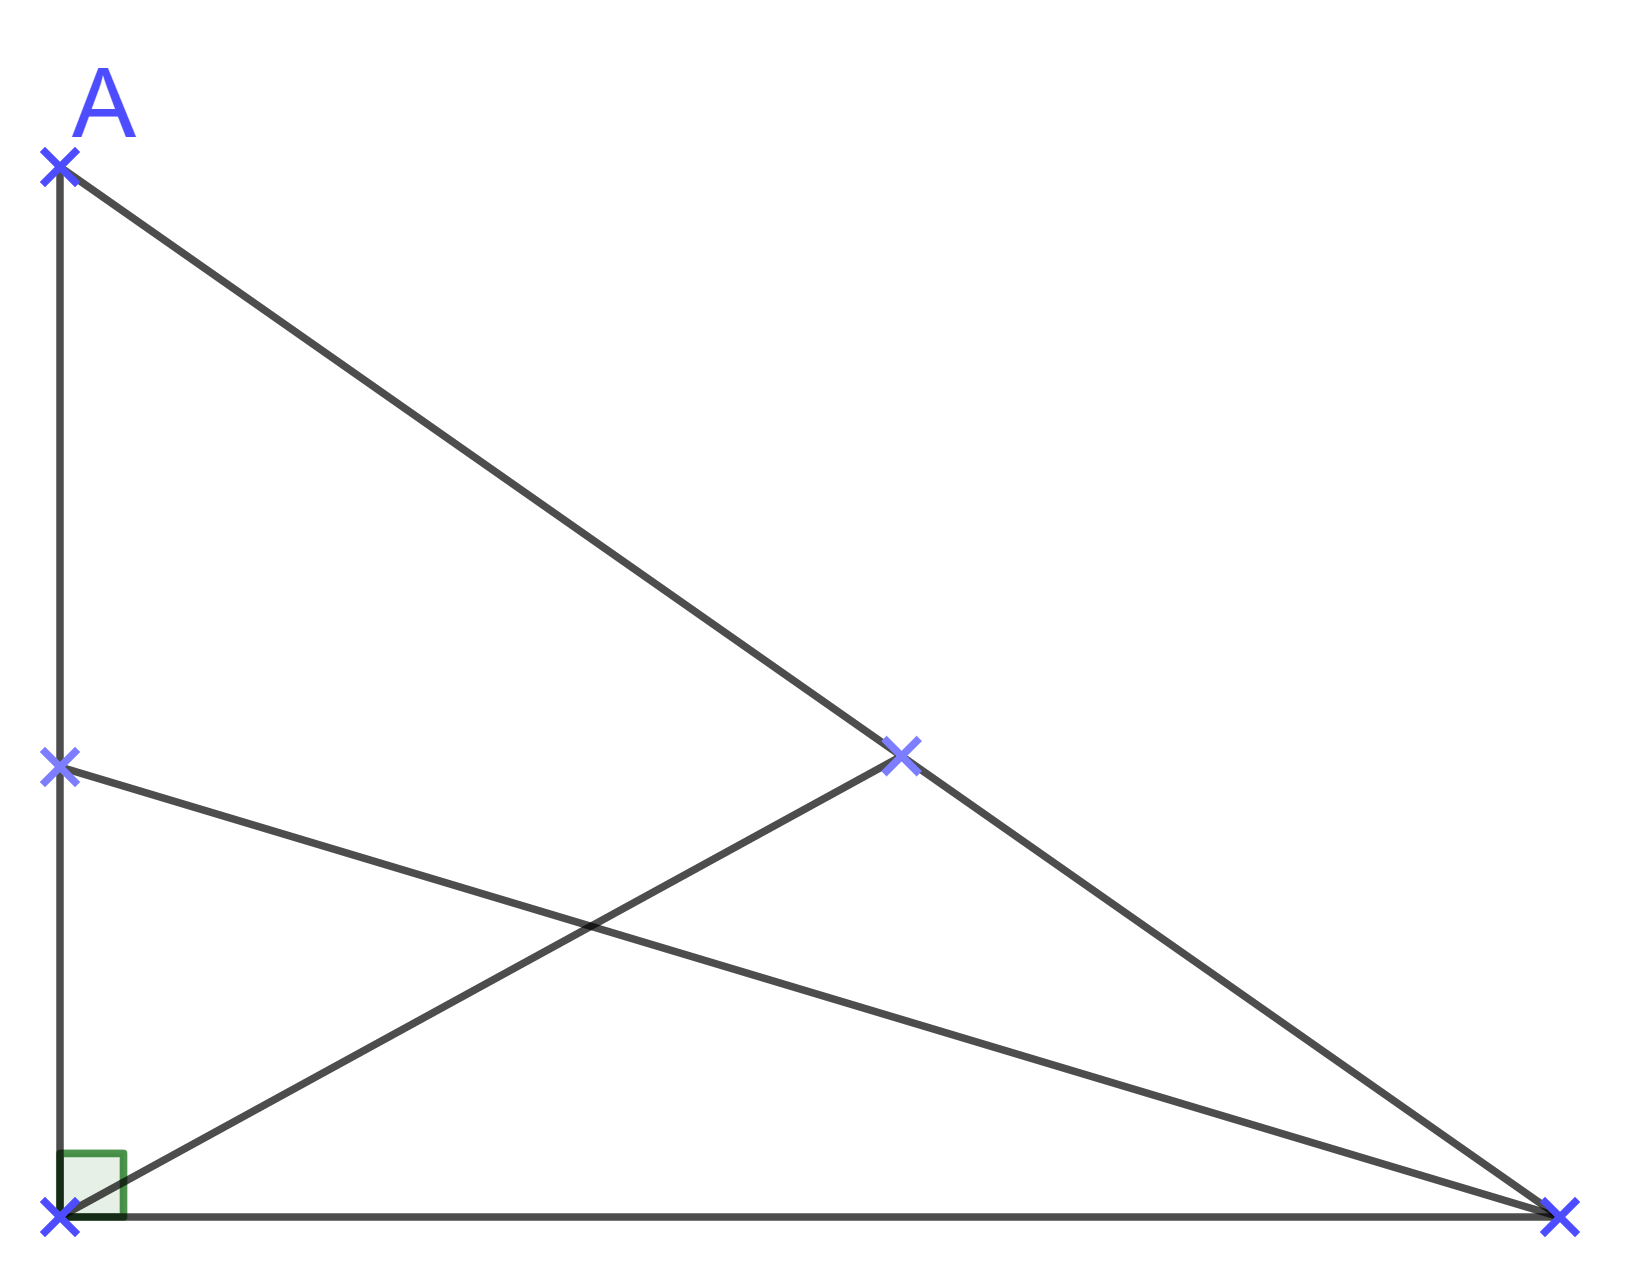
\includegraphics[scale=0.15]{img/ex1}
		\end{center}
		
		\begin{itemize}
			\item $\widehat{ABC}$ est droit;
			\item $\widehat{BDC}$ est aigu;
			\item $\widehat{CEB}$ est obtus;
		\end{itemize}
	\end{multicols}
	
	
\end{questions}

